\documentclass{standalone}
\usepackage{tikz-network}
\begin{document}
	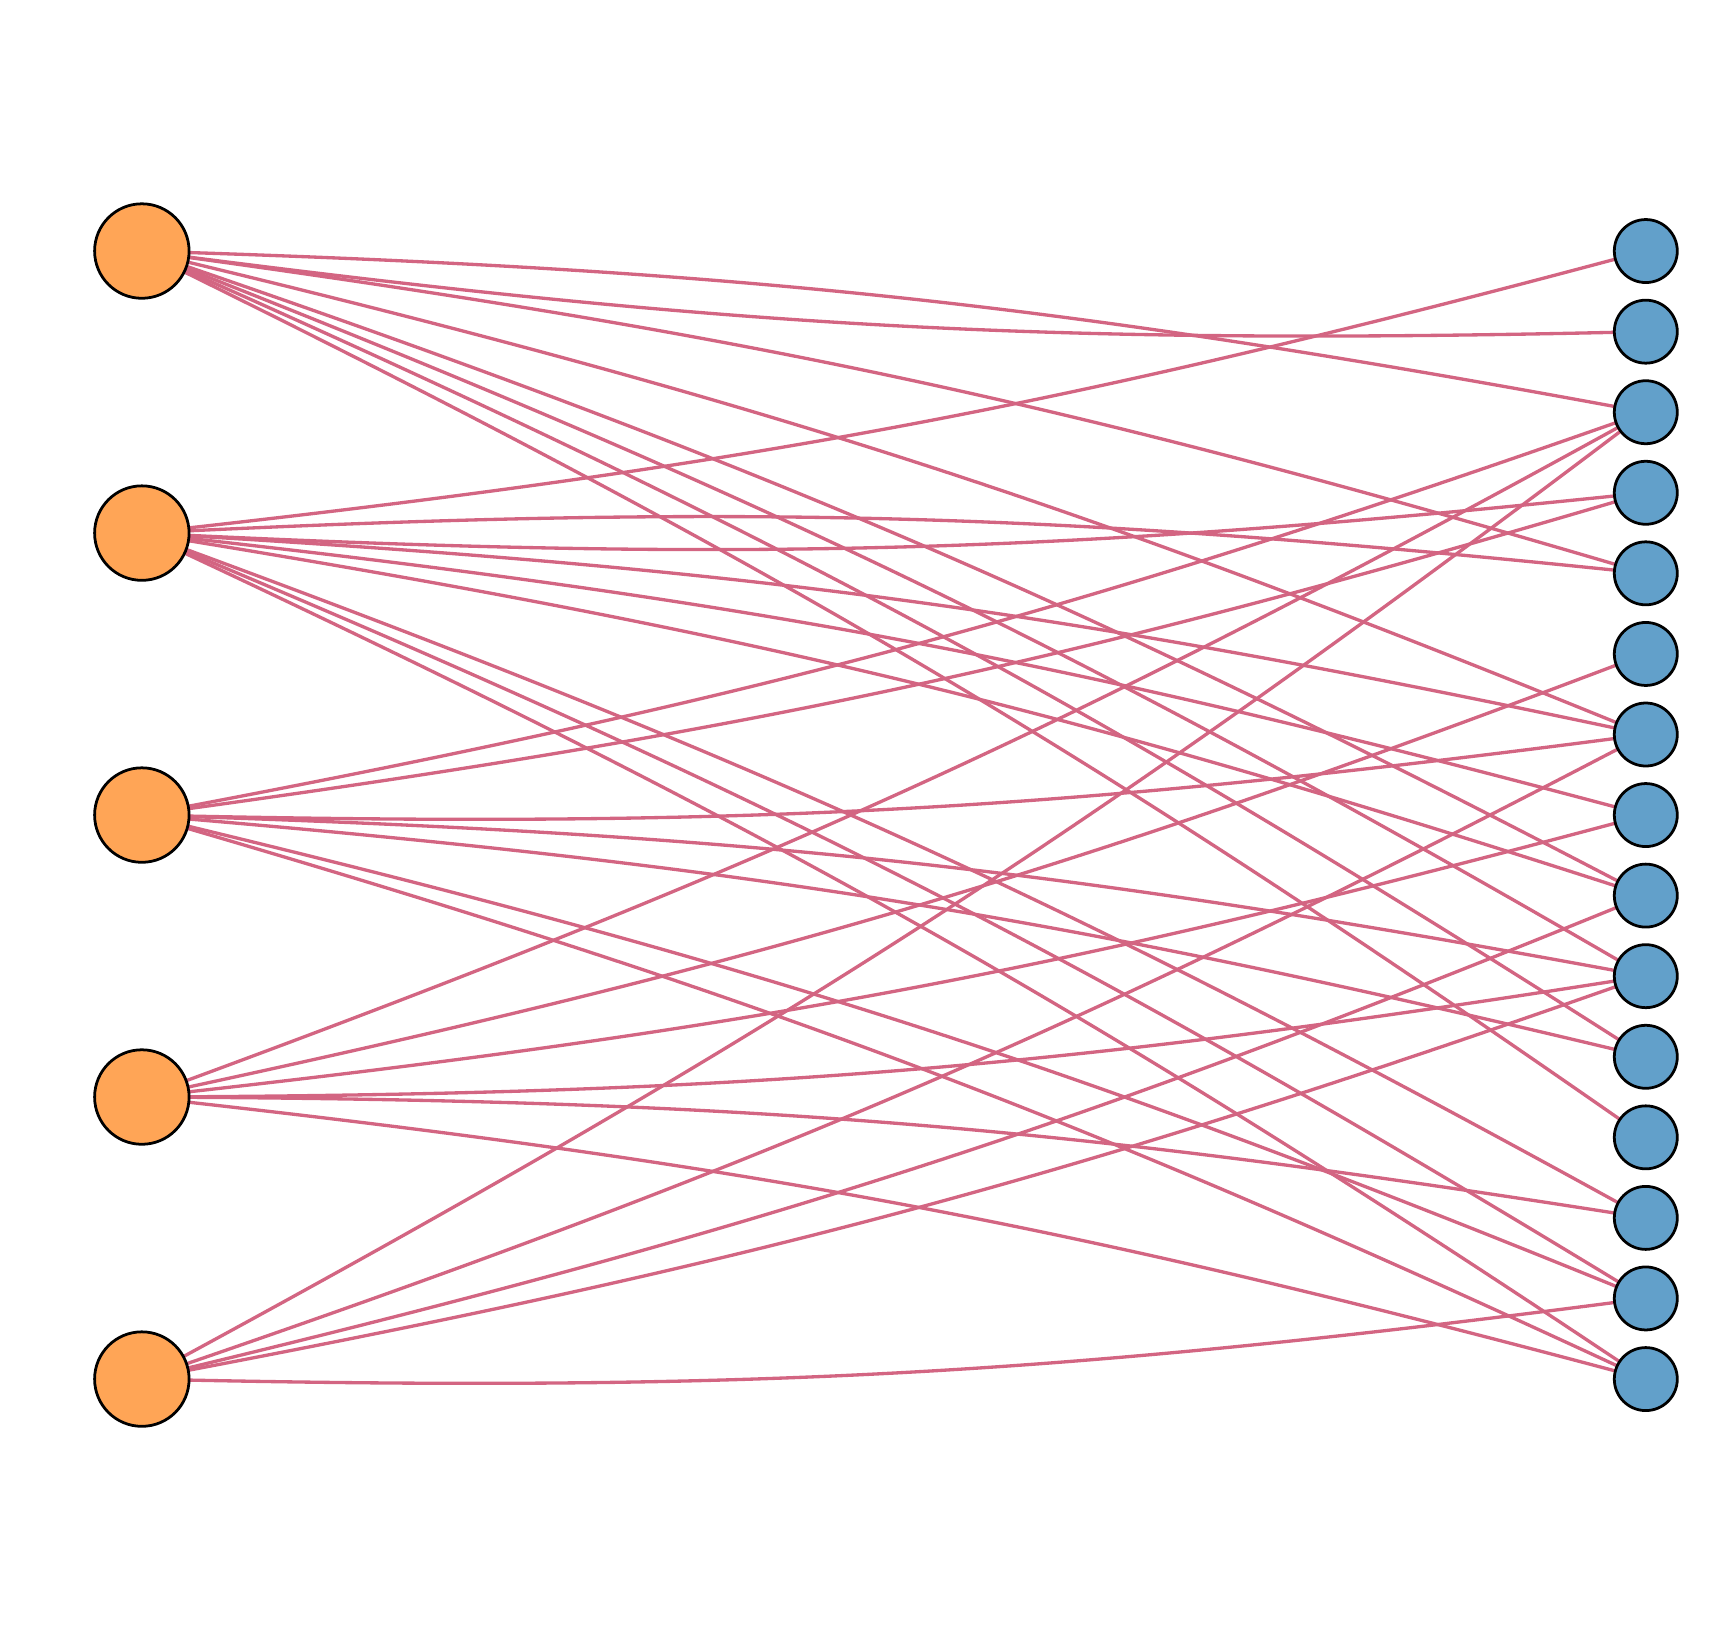
\begin{tikzpicture}
		\clip (-1,0) rectangle (20.0,20.0);
		\Vertex[x=19.550,y=2.837,size=0.8,color={31.0,119.0,180.0},opacity=0.7,RGB]{0}
		\Vertex[x=0.450,y=2.837,size=1.2,color={255.0,127.0,14.0},opacity=0.7,RGB]{1}
		\Vertex[x=19.550,y=3.861,size=0.8,color={31.0,119.0,180.0},opacity=0.7,RGB]{2}
		\Vertex[x=19.550,y=4.884,size=0.8,color={31.0,119.0,180.0},opacity=0.7,RGB]{3}
		\Vertex[x=0.450,y=6.419,size=1.2,color={255.0,127.0,14.0},opacity=0.7,RGB]{4}
		\Vertex[x=19.550,y=5.907,size=0.8,color={31.0,119.0,180.0},opacity=0.7,RGB]{5}
		\Vertex[x=19.550,y=6.930,size=0.8,color={31.0,119.0,180.0},opacity=0.7,RGB]{6}
		\Vertex[x=19.550,y=7.954,size=0.8,color={31.0,119.0,180.0},opacity=0.7,RGB]{7}
		\Vertex[x=0.450,y=10.000,size=1.2,color={255.0,127.0,14.0},opacity=0.7,RGB]{8}
		\Vertex[x=19.550,y=8.977,size=0.8,color={31.0,119.0,180.0},opacity=0.7,RGB]{9}
		\Vertex[x=19.550,y=10.000,size=0.8,color={31.0,119.0,180.0},opacity=0.7,RGB]{10}
		\Vertex[x=19.550,y=11.023,size=0.8,color={31.0,119.0,180.0},opacity=0.7,RGB]{11}
		\Vertex[x=19.550,y=12.046,size=0.8,color={31.0,119.0,180.0},opacity=0.7,RGB]{12}
		\Vertex[x=19.550,y=13.070,size=0.8,color={31.0,119.0,180.0},opacity=0.7,RGB]{13}
		\Vertex[x=0.450,y=13.581,size=1.2,color={255.0,127.0,14.0},opacity=0.7,RGB]{14}
		\Vertex[x=19.550,y=14.093,size=0.8,color={31.0,119.0,180.0},opacity=0.7,RGB]{15}
		\Vertex[x=19.550,y=15.116,size=0.8,color={31.0,119.0,180.0},opacity=0.7,RGB]{16}
		\Vertex[x=0.450,y=17.163,size=1.2,color={255.0,127.0,14.0},opacity=0.7,RGB]{17}
		\Vertex[x=19.550,y=16.139,size=0.8,color={31.0,119.0,180.0},opacity=0.7,RGB]{18}
		\Vertex[x=19.550,y=17.163,size=0.8,color={31.0,119.0,180.0},opacity=0.7,RGB]{19}
		\Edge[,lw=1.2,color={211,101,130},bend=-4.289,RGB](0)(4)
		\Edge[,lw=1.2,color={211,101,130},bend=-4.289,RGB](0)(8)
		\Edge[,lw=1.2,color={211,101,130},bend=-4.289,RGB](0)(14)
		\Edge[,lw=1.2,color={211,101,130},bend=-4.289,RGB](1)(2)
		\Edge[,lw=1.2,color={211,101,130},bend=-4.289,RGB](1)(7)
		\Edge[,lw=1.2,color={211,101,130},bend=-4.289,RGB](1)(9)
		\Edge[,lw=1.2,color={211,101,130},bend=-4.289,RGB](1)(11)
		\Edge[,lw=1.2,color={211,101,130},bend=-4.289,RGB](1)(16)
		\Edge[,lw=1.2,color={211,101,130},bend=-4.289,RGB](2)(8)
		\Edge[,lw=1.2,color={211,101,130},bend=-4.289,RGB](2)(14)
		\Edge[,lw=1.2,color={211,101,130},bend=-4.289,RGB](3)(4)
		\Edge[,lw=1.2,color={211,101,130},bend=-4.289,RGB](3)(14)
		\Edge[,lw=1.2,color={211,101,130},bend=-4.289,RGB](4)(7)
		\Edge[,lw=1.2,color={211,101,130},bend=-4.289,RGB](4)(10)
		\Edge[,lw=1.2,color={211,101,130},bend=-4.289,RGB](4)(12)
		\Edge[,lw=1.2,color={211,101,130},bend=-4.289,RGB](4)(16)
		\Edge[,lw=1.2,color={211,101,130},bend=-4.289,RGB](5)(17)
		\Edge[,lw=1.2,color={211,101,130},bend=-4.289,RGB](6)(8)
		\Edge[,lw=1.2,color={211,101,130},bend=-4.289,RGB](6)(17)
		\Edge[,lw=1.2,color={211,101,130},bend=-4.289,RGB](7)(8)
		\Edge[,lw=1.2,color={211,101,130},bend=-4.289,RGB](7)(17)
		\Edge[,lw=1.2,color={211,101,130},bend=-4.289,RGB](8)(11)
		\Edge[,lw=1.2,color={211,101,130},bend=-4.289,RGB](8)(15)
		\Edge[,lw=1.2,color={211,101,130},bend=-4.289,RGB](8)(16)
		\Edge[,lw=1.2,color={211,101,130},bend=-4.289,RGB](9)(14)
		\Edge[,lw=1.2,color={211,101,130},bend=-4.289,RGB](9)(17)
		\Edge[,lw=1.2,color={211,101,130},bend=-4.289,RGB](10)(14)
		\Edge[,lw=1.2,color={211,101,130},bend=-4.289,RGB](11)(14)
		\Edge[,lw=1.2,color={211,101,130},bend=-4.289,RGB](11)(17)
		\Edge[,lw=1.2,color={211,101,130},bend=-4.289,RGB](13)(14)
		\Edge[,lw=1.2,color={211,101,130},bend=-4.289,RGB](13)(17)
		\Edge[,lw=1.2,color={211,101,130},bend=-4.289,RGB](14)(15)
		\Edge[,lw=1.2,color={211,101,130},bend=-4.289,RGB](14)(19)
		\Edge[,lw=1.2,color={211,101,130},bend=-4.289,RGB](16)(17)
		\Edge[,lw=1.2,color={211,101,130},bend=-4.289,RGB](17)(18)
	\end{tikzpicture}
\end{document}